\documentclass[../thesis]{subfiles}
\graphicspath{{\subfix{../figures/}}}

\begin{document}
\chapter{User Study}\label{ch:evaluation}

\lettrine[lines=3]{\textcolor{Maroon}{D}}{espite} having already done a technical evaluation in \cref{sec:techeval}, it is usually also a good idea to compare new approaches with existing state-of-the-art tools in a user study.
In our case, we want to compare \SEE{}'s \gls{lsp}-generated \glspl{city} with the \glspl{capability} a normal \gls{lsp}-enabled \gls{ide} offers.
For the latter, the Microsoft-developed \gls{ide} \gls{vscode} is a good fit, given that the \glsentrylong{lsp} itself originates here (see \cref{sec:lsp}) and that it still has a deep integration with it.

First, we will outline the general aim of this study by going over some existing related research, explaining important aspects of \gls{vscode}, and then enumerating our hypotheses.
Next, we will explain the details of the design of the study itself, before analyzing its results with the \participants{} participants in detail.
Finally, we describe some relevant threats to validity.

As a quick aside before we begin, we will frequently use \glspl{violin} in this chapter to visualize datasets, especially to visually compare two datasets against one another.
To estimate the probability density for the plots, we need to use a non-parametric kernel density estimation (since we do not know which shape the underlying distribution has)---for the kernel itself, we simply use a gaussian function, but a much more important question is the choice of the bandwidth parameter~\cite{heidenreich2013}.
Here, we use an algorithm by \textcite{sheather1991} that has been improved to be made more performant and handle multimodal distributions better by \textcite{botev2010a}:
The \emph{Improved Sheather--Jones} method, which is a robust choice when one cannot assume normality~\cite{akinshin2020}.
As the algorithm for this method, we use \tt{KDEpy}~\cite{odland2018}, whose implementation of the method is based on \textcite[326--328]{kroese2011}.
A drawback here is that this algorithm does not necessarily converge.
In those cases, we fall back to using Silverman's rule of thumb~\cite{silverman1986}, the implementation of which is integrated in the library we use to draw these plots~\cite{callil-soares2024}.

\section{Plan}  % TODO: Different title?
Our main aim here is to answer our second research question that we defined in \cref{sec:goals}:
\begin{displayquote}
	Are \glspl{city} a suitable means to present \gls{lsp} information to developers as compared to \glspl{ide} + tables (on the dimensions of speed, accuracy, and usability)?
\end{displayquote}

To empirically evaluate this research question, we will devise a series of short software engineering related tasks.
Participants then get randomly assigned to either use \SEE{} (along with our implementation from \cref{ch:implementation}) or \gls{vscode} (with an active \gls{ls}).
However, evaluating the supported \glspl{capability} (see \cref{tab:capabilities}) in this way turns out to be quite difficult---for example, how would one evaluate the \emph{Hover} \gls{capability}, let alone features like \glspl{token} which are almost identically implemented across \SEE{} and \gls{vscode}?
For this reason, we will abstain from incorporating the \gls{window}-related \glspl{capability} from \cref{sec:intowindow}.
Limiting ourselves, then, to the \gls{city}-related changes from \cref{sec:intocity}, we have:
\begin{enumerate}
	\item \emph{Diagnostics} being displayed as erosion icons above corresponding nodes.\\
	      $\Rightarrow$ This feature was essentially already evaluated in my bachelor's thesis, albeit with the Axivion Dashboard as a data source instead of \gls{lsp}~\cite{galperin2021,galperin2022}.
	\item \emph{Hover} details being displayed when the user hovers the mouse above a node.\\
	      $\Rightarrow$ Since this is used here almost identically as in \glspl{window}, it does not make much sense to compare it against \gls{vscode}.
	\item \emph{Go to location}, \emph{references}, and \emph{call/type hierarchy} being used for rendered edges and context menu actions.\\
	      $\Rightarrow$ The context menu actions are not interesting to evaluate for the same reasons as above, though this does not apply to the generated edges.
\end{enumerate}

It appears that the only \glspl{capability} that are reasonably evaluable in a user study of this form are actually the ones used in the generation of the \gls{city} in \cref{sec:generate}.
Besides, the bulk of the implementation pertains to the generation of \glspl{city}, so it makes sense to focus on them here.
As a result, the user study is now actually of a form (directly comparing \glspl{city} against \glspl{ide}) that has been researched in previous literature before, so let us take a look at that research first before designing our own study.

\subsection{Existing Research}\label{subsec:research}
Across various bachelor's and master's theses, a number of user studies have been performed about \SEE{}'s usability in various aspects~\cite{davidwagner2020, felixgaebler2021, hannesmasuch2020, kevindoehl2020, maximilianwick2022, michelkrause2024, robertbohnsack2020, rubensmidt2021} as well as about its effectiveness compared to traditional tools~\cite{galperin2021, lennartkipka2020, moritz, nicoweiser2021, rohlfing2024, schramm2022, sulanabubakarov2021, yannisrohloff2021}.
Especially relevant among the latter kind of studies are the three that compare \SEE{} with traditional \glspl{ide}, as that is very close to our own planned evaluation.
Two of these evaluate debugging capabilities that have been implemented into \SEE{}:
\textcite{lennartkipka2020} compares those with Eclipse\footnote{
	\web{https://www.eclipse.org/}{2024-11-17}
}'s debugger, while \textcite{rohlfing2024} uses the debugger of \gls{vscode} as a baseline.
The final of these studies has \textcite{schramm2022} compare pure \gls{ide} usage (in this case, Microsoft's Visual Studio) with a combination of Visual Studio and \SEE{} in which Visual Studio has a plugin setup that integrates it with \SEE{}.
The result here was a significant improvement for usability and a partial improvement for efficiency in favor of the combination of Visual Studio and \SEE{}.
Almost all of these \SEE{}-related studies measure its usability in the form of the \gls{sus}---which we will do in our own study, as well.
I have collected the existing scores of those studies in a \gls{violin} in \cref{fig:seesus}.

\begin{figure}
	\begin{center}
		\begin{tikzpicture}
			\violinsetoptions[data points,scaled,averages]{
				xmin=0,xmax=2,
				ymin=55,ymax=95,
				ylabel={SUS},
				ymajorgrids=true
			}

			\violinplot[%
				index=sus,%
				col sep=tab,%
				color=Maroon,%
				dataset size=3pt,%
				average size=5pt,%
				average opacity=0.8,%
				average color=black,%
				dataset opacity=0.8,%
				dataset jitter=0.1,%
				relative position=1,%
				bandwidth=2.1269,%
				average fill opacity=0.5,%
				average fill=ForestGreen,%
				average mark=otimes*,%
				dataset color=black,%
				dataset fill=black,%
				dataset fill opacity=0.5,%
				label={SEE}
			]{analysis/dat/sus.dat}
		\end{tikzpicture}
	\end{center}
	\caption{\Gls{sus} results for \SEE{} across various studies~\cite{davidwagner2020, felixgaebler2021, galperin2021, hannesmasuch2020, kevindoehl2020, lennartkipka2020, maximilianwick2022, michelkrause2024, moritz, nicoweiser2021, robertbohnsack2020, rohlfing2024, rubensmidt2021, schramm2022, sulanabubakarov2021, yannisrohloff2021}.}\label{fig:seesus}
\end{figure}

Outside of \SEE{}, there are a number of other \gls{city} implementations, such as \emph{CodeCity}~\cite{wettel2007} or \emph{Software World}~\cite{knight2000} (see also the overview by \textcite{jeffery2019}).
In their evaluations, these papers often compare different platforms (such as Desktop to VR/AR)~\cite[\eg,][]{merino2017,fittkau2015, merino2018}, but as with the \SEE{}-related theses above, we are most interested in those that have controlled experiments comparing a \gls{city} implementation with a traditional \gls{ide}.

One such study was done by \textcite{wettel2011} and compares \emph{CodeCity} against the Eclipse \gls{ide}, with the caveat that participants using Eclipse can also access an Excel spreadsheet of software metrics, as the \gls{city} implementation would otherwise have an unfair advantage.
He based his study on an extensive survey of existing empirical work on software visualization, constructing a "wishlist" of desiderata for such studies~\cite[chapter 7]{wettel2011}.
We will refer back to this wishlist, and to his experiment design in general, in \cref{sec:design} for our own study.
The study was later replicated by \textcite{romano2019} with a subset of tasks.

Similarly, \textcite{mortara2024} supplied \gls{csv} files for \gls{ide} users in a comparison against \emph{VariCity}, although here, participants were allowed to choose whatever \gls{ide} they are most comfortable with.
\textcite{mehra2020} gave participants who were using Eclipse an additional 2D graph tool when evaluating the augmented reality \textsc{XRaSE} \gls{city} visualization.
On the other hand, the category of comparative user studies between \glspl{city} and \glspl{ide} without any other helper tools (which our own study will also fall into) includes ones by \textcite{khaloo2017,rohlfing2024,lennartkipka2020}.
The results of their experiments, and all others cited here, are listed in the color-coded \cref{tab:compresults}.

\colorlet{LightMaroon}{Maroon!30!white}
\colorlet{LightBlue}{Cyan!30!white}

% Maybe also for non-IDE comp for SEE?
% yellow: mixed, gray: no sig. diff., (light) maroon favor of CC, (light) blue: favor of IDE
% with legend

\newcommand{\reside}[1]{\cellcolor{Blue}\textcolor{White}{#1}}
\newcommand{\rescc}[1]{\cellcolor{Maroon}\textcolor{White}{#1}}
\newcommand{\residel}[1]{\cellcolor{LightBlue}#1}  % e.g., < 50% of tasks
\newcommand{\resccl}[1]{\cellcolor{LightMaroon}#1}
\newcommand{\resmixed}[1]{\cellcolor{Goldenrod}#1}  % Mixed between tasks
\newcommand{\resnone}[1]{\cellcolor{Gray!70!white}No diff.}  % No sig. diff.
% White: not measured
\newcommand{\resna}[1]{\textcolor{Gray}{\textit{N/A}}}

\begin{table}
	\begin{center}
		\caption{Results of various studies comparing \glspl{city} (CC) against \glspl{ide}. $x/y$ indicates an advantage in $x$ out of $y$ tasks or questions.}\label{tab:compresults}
		{
			\footnotesize
			\def\arraystretch{1.3}
			\begin{tabular}{|l|l|l|l|l|l|l|}
				\hline
				Study                   & $n$ & Correctness         & Time                           & Usability                      & \gls{ide}          & Code City      \\ \hline
				\cite{wettel2011}       & 45  & \rescc{$p = 0.001$} & \rescc{$p=0.043$}              & \resna{}                       & Eclipse + metrics  & CodeCity       \\ \hline
				\cite{khaloo2017}       & 28  & \resna{}            & \reside{$3/5$ IDE}             & \resccl{$6/20$ CC; $1/20$ IDE} & Visual Studio (VS) & Code Park      \\ \hline
				\cite{romano2019}       & 54  & \rescc{$p= 0.005$}  & \rescc{$p < 0.001\%$}          & \resnone{}                     & Eclipse + metrics  & Code2City      \\ \hline
				\cite{lennartkipka2020} & 10  & \resnone{}          & \resnone{}                     & \resnone{}                     & Eclipse            & \SEE{}         \\ \hline
				\cite{mehra2020}        & 20  & \rescc{$p= 0.005$}  & \resccl{$3/5$ CC; $1/5$ IDE}   & \resccl{Preliminary only}      & Eclipse + 2D graph & \textsc{XRaSE} \\ \hline
				\cite{galperin2022}     & 20  & \residel{$2/6$ IDE} & \rescc{$4/6$ CC}               & \reside{$p = 0.028$}           & Axivion Dashboard  & \SEE{}         \\ \hline
				\cite{schramm2022}      & 10  & \resnone{}          & \resccl{$1/3$ CC}              & \rescc{$p = 0.002$}            & VS + Axivion       & VS + \SEE{}    \\ \hline
				\cite{mortara2024}      & 49  & \rescc{$6/11$ CC}   & \resccl{$4/11$ CC; $1/11$ IDE} & \resccl{$4/11$ CC}             & Various + metrics  & VariCity       \\ \hline
			\end{tabular}
		}
		\caption*{\footnotesize Legend: \legendsquare{Maroon} \Gls{city} advantage, \legendsquare{LightMaroon} Slight \gls{city} advantage, \legendsquare{Blue} \Gls{ide} advantage, \mbox{\legendsquare{LightBlue} Slight \gls{ide} advantage}, \mbox{\legendsquare{Gray} No significant difference}, \mbox{{\normalsize $\Box$} Not measured}
		}
	\end{center}
\end{table}


\subsection{VSCode}\label{subsec:vscode}

\begin{figure}[htbp]
	\begin{center}
		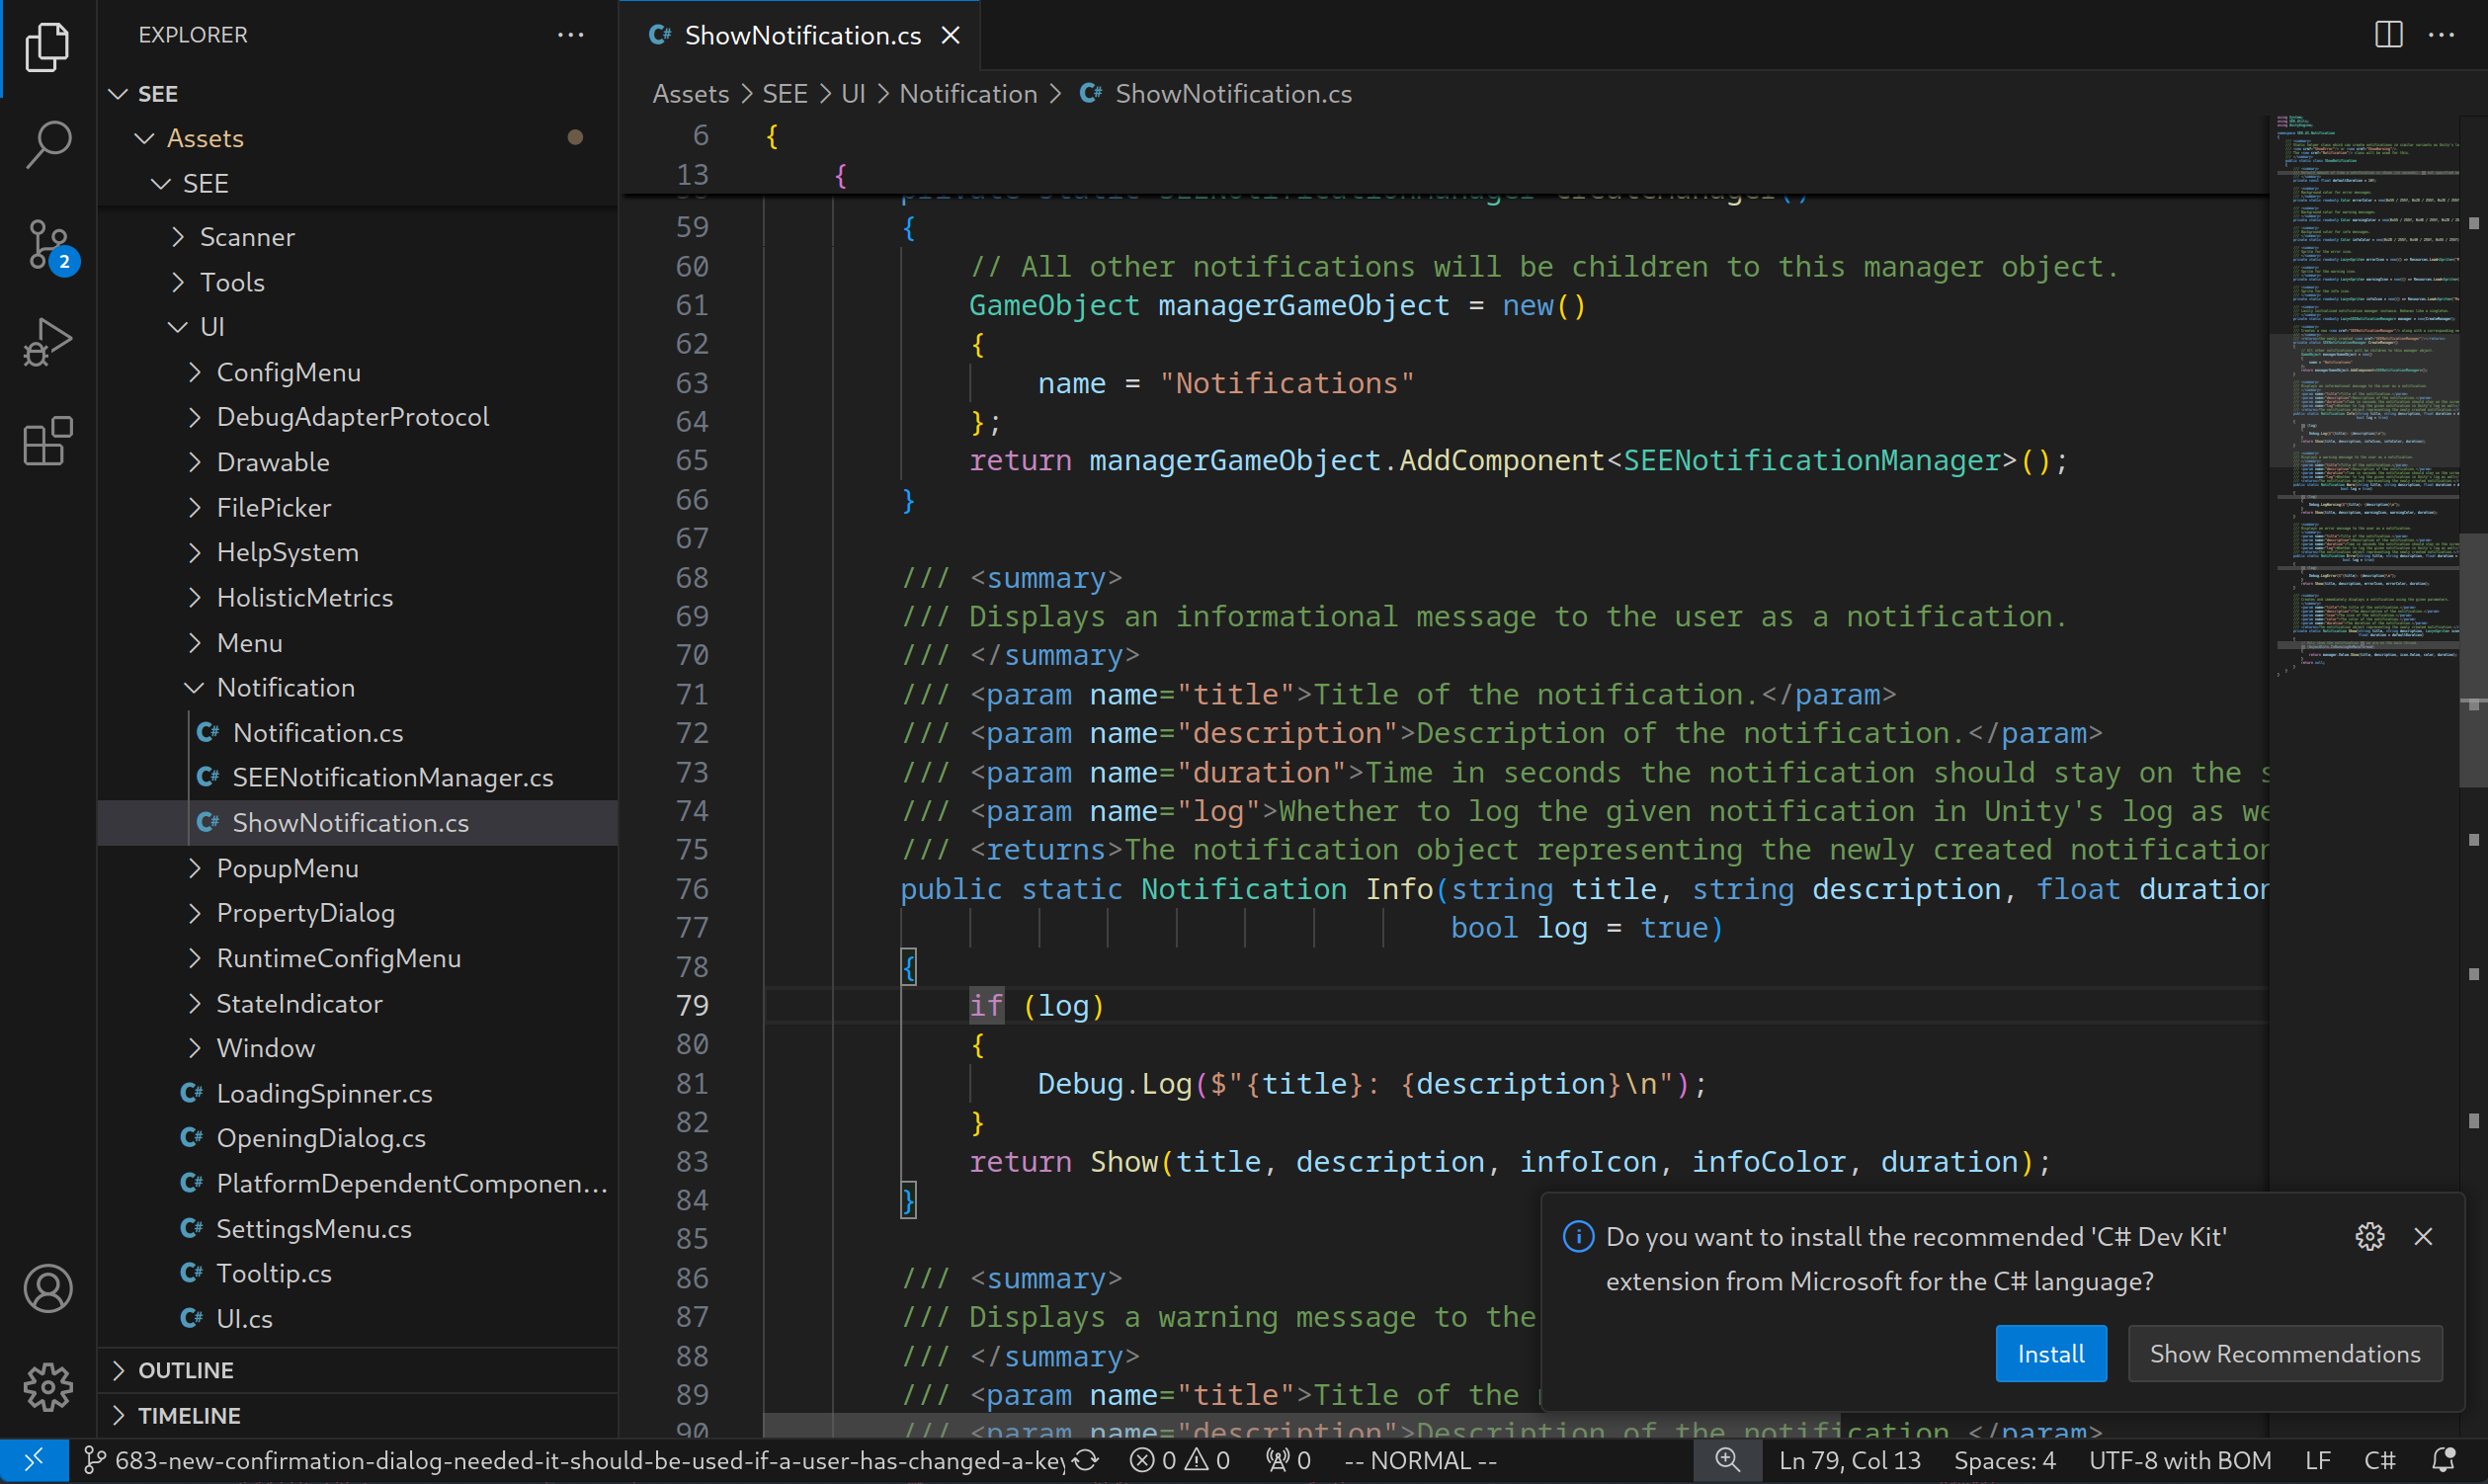
\includegraphics[width=0.95\textwidth]{VSCode}
	\end{center}
	\caption{Screenshot of the main \gls{ui} of \gls{vscode}.}\label{fig:vscode}
\end{figure}

Here, we will very briefly go over \gls{vscode} as the tool that we will compare \SEE{} against.
A screenshot of \gls{vscode} is provided in \cref{fig:vscode}.
On the left side, we can see the filesystem hierarchy of the open project, in the middle is the code itself, and on the right is a minimap as a quick overview of the current file's code.
\gls{vscode} also has an extension system in place with which \glspl{ls} and other enhancements to the editor can be easily installed---for example, we can see a notification in the bottom right prompting the user to install the C\# extension.

\begin{figure}[htbp]
	\begin{center}
		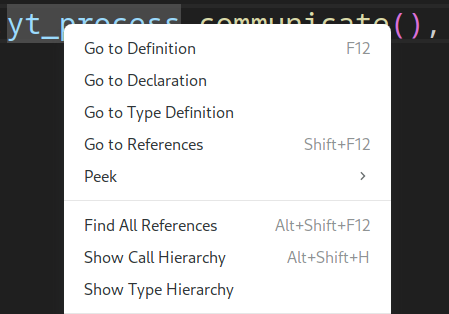
\includegraphics[width=0.5\textwidth]{VSCode-menu}
	\end{center}
	\caption{Screenshot of (the beginning of) \gls{vscode}'s context menu for code identifiers.}\label{fig:vscode_menu}
\end{figure}

It is also possible to quickly find files with the \keystroke{Ctrl} + \keystroke{P} shortcut, which pops up a menu with a live search through all filenames in the project.
The analogue in \SEE{} is the tree view which was showcased in \cref{sec:intocity}.
Also shown in that chapter was a context menu with various options to make use of the \gls{lsp} "go to location" \glspl{capability}.
\Gls{vscode} has a very similar context menu when right-clicking code identifiers, which is displayed in \cref{fig:vscode_menu}.
Additionally, \gls{vscode} users can also jump to the definition of a symbol by holding down \keystroke{Ctrl} and clicking on that symbol, the same as in \cref{sec:intowindow}.

However, a feature of \SEE{} which \emph{does not} have a clear alternative in \gls{vscode} is the ability to quickly be able to tell certain metrics, such as the number of methods in a file.
In \SEE{}, we could simply visualize that by encoding it as the size of each building, but in \gls{vscode}, participants would need to manually count each method, so to remedy this, we offer a table with such metrics.
The table is hosted on Google Spreadsheets\footnote{
	\web{https://docs.google.com/spreadsheets/d/1Z2AQDk2-XeVBB1kAtcpc18mFkPI5ZSsSz\_yOwS4pQ88}{2024-11-20} and \web{https://docs.google.com/spreadsheets/d/1erJZTwYtG-CQfZJPT-zt-chX\_VHL9jLrVfWAWZMFvEo}{2024-11-20}.
} and can be sorted by any column as well as searched.

\subsection{Hypotheses}\label{subsec:hypotheses}

To answer \textsf{RQ2} (see \cref{sec:goals}), we would like to know whether there is any significant difference between the approaches on the dimensions of \emph{speed}, \emph{correctness}, and \emph{usability}, similar to most other studies mentioned in \cref{subsec:research}.
We will now create more concrete hypotheses for each of these dimensions.

\begin{enumerate}[label=\alph*)]
	\item \textbf{Correctness}: We call the correctness $C_S$ for tasks done in \SEE{} and $C_V$ for tasks done in \gls{vscode}.
	      This will be either a categorical variable with two possible values (\ie, correct or incorrect) or a rational number indicating the percentage of correct answers within a task.
	      \begin{itemize}
		      \item \emph{Null hypothesis} $H_{a_0}$:
		            The correctness when using \SEE{} is the same as when using \gls{vscode}: $C_S = C_V$.
		      \item \emph{Alternative hypothesis} $H_{a_1}$:
		            The correctness when using \SEE{} is different when using \gls{vscode}: $C_S \neq C_V$.
	      \end{itemize}
	\item \textbf{Speed}: We call the time it takes to finish a task $t_S$ for \SEE{} and $t_V$ for \gls{vscode}.
	      \begin{itemize}
		      \item \emph{Null hypothesis} $H_{b_0}$:
		            The time it takes to solve a task when using \SEE{} is the same as when using \gls{vscode}: $t_S = t_V$.
		      \item \emph{Alternative hypothesis} $H_{b_1}$:
		            The time it takes to solve a task when using \SEE{} is different when using \gls{vscode}: $t_S \neq t_V$.
	      \end{itemize}
\end{enumerate}

For the \textbf{usability}, we need to differentiate between the \gls{poststudy} \gls{sus} we use to evaluate the usability of the system as a whole, and the reduced 2-item \gls{posttask} \gls{asq} we use after each task (see \cref{subsec:question}).

\begin{enumerate}[resume,label=\alph*)]
	\item \textbf{\gls{sus}}:
	      We call the \gls{sus} score for \SEE{} $S_S$ and the one for \gls{vscode} $S_D$.
	      \begin{itemize}
		      \item \emph{Null hypothesis} $H_{c_0}$:
		            The \gls{sus} score for \SEE{} is the same as the \gls{sus} score for \gls{vscode}: $S_S = S_V$.
		      \item \emph{Alternative hypothesis} $H_{c_1}$:
		            The \gls{sus} score for \SEE{} is different from the \gls{sus} score for \gls{vscode}: $S_S \neq S_V$.
	      \end{itemize}
	\item \textbf{\gls{asq}}:
	      We need to once again differentiate between the two aspects that the \gls{asq} measures.
	      \begin{enumerate}[label=\roman*)]
		      \item We call the \gls{asq} score for \emph{complexity}\footnote{
			            Note that a higher score here means a lower amount of complexity.
		            } $A^c_S$ for \SEE{} and $A^c_V$ for \gls{vscode}.
		            \begin{itemize}
			            \item \emph{Null hypothesis} $H_{d_0}$:
			                  The \gls{asq} score for complexity when using \SEE{} is the same as when using \gls{vscode}.
			            \item \emph{Alternative hypothesis} $H_{d_1}$:
			                  The \gls{asq} score for complexity when using \SEE{} is different when using \gls{vscode}.
		            \end{itemize}
		      \item We call the \gls{asq} score for \emph{effort}\footnote{
			            Again, a higher score indicates less required effort.
		            } $A^e_S$ for \SEE{} and $A^e_V$ for \gls{vscode}.
		            \begin{itemize}
			            \item \emph{Null hypothesis} $H_{e_0}$:
			                  The \gls{asq} score for effort when using \SEE{} is the same as when using \gls{vscode}.
			            \item \emph{Alternative hypothesis} $H_{e_1}$:
			                  The \gls{asq} score for effort when using \SEE{} is different when using \gls{vscode}.
		            \end{itemize}
	      \end{enumerate}
\end{enumerate}

We will use a significance level of $\alpha = 0.05$ for \fxwarning*{Except maybe effects!}{all} of our tests.

\section{Design}\label{sec:design}
\fxfatal{}

\fxnote{Refer back to Wettel's wish list}

\subsection{Questionnaire}\label{subsec:question}
\fxfatal{}

\subsection{Tasks}
\fxfatal{}

\section{Results}
\fxfatal{}

\subsection{Demographics}
\fxfatal{}

%
% \violinab{age}{Age}{20}{40}
%
% \violinab{total-time}{Total Participation Time (hours)}{0}{5}
%
% % TODO: ordinal data
%
% \violinsv{a1-time}{Time (Minutes)}{0}{20}
% \violinsv{a2-time}{Time (Minutes)}{0}{20}
% \violinsv{a3-time}{Time (Minutes)}{0}{10}
% \violinsv{a4-time}{Time (Minutes)}{0}{10}
% \violinsv{a5-time}{Time (Minutes)}{0}{20}
% \violinsv{a6-time}{Time (Minutes)}{0}{10}
%
% \violinsus{}

% \begin{tikzpicture}
% 	\violinsetoptions[data points,scaled,averages]{
% 		xmin=0,xmax=3,
% 		ymin=50,ymax=100,
% 		xlabel={Sys},
% 		xlabel style={
% 				yshift={-0.5cm},
% 			},
% 		ylabel={SUS},
% 		ymajorgrids=true
% 	}
%
% 	\violinplot[%
% 		index=sus,%
% 		col sep=tab,%
% 		color=Maroon,%
% 		dataset size=3pt,%
% 		average size=4pt,%
% 		average opacity=0.8,%
% 		average color=black,%
% 		dataset opacity=0.8,%
% 		dataset jitter=0.1,%
% 		relative position=1,%
% 		average fill opacity=0.5,%
% 		average fill=ForestGreen,%
% 		average mark=otimes*,%
% 		dataset color=black,%
% 		dataset fill=black,%
% 		dataset fill opacity=0.5,%
% 		label={SEE}
% 	]{analysis/dat/sus.dat}
% \end{tikzpicture}

\subsection{Correctness}
\fxfatal{}

\subsection{Time}
\fxfatal{}

\subsection{Usability}
\fxfatal{}

\fxfatal{Also a section on the effect of experience (and others)}

\subsection{Comments}
\fxfatal{}

\section{Threats to Validity}
\fxfatal{}

\section{Interim Conclusion}  % Or maybe just recap?
\fxfatal{}
